\section{Introduction}
The Semantic Web is often understood as an immense engineering project that relies on a relatively small set of broadly accepted guidelines, which in their turn  will lead to a large degree of interoperability. However, the existing inventory of representational constructs for web knowledge bases has already given rise to a variety of patterns and nuances in data modeling. Analyzing the ways in which different people and communities spontaneously design their data-modeling schemes, many of which have already been broadly used, should be a legitimate part of the Semantic Web movement.

One part of such empirical research that we are currently pursuing is the analysis of occurrence, structure, and role of \emph{ontology-embedded code lists}, which can be approximately characterized as (relatively) closed sets of co-created syntactic individuals meant to be used as values of certain properties defined by the ontology.
%in RDF knowledge bases, which we view as a distinct third component of the web knowledge base, together with ontologies in the form of vocabularies and schemas, and instance-level knowledge graphs that are fundamentally nothing else but linked datasets. 
%\section{Motivation} 
%Unlike the ontology schemas inside which they reside, embedded code lists are: 1) syntactically expressed at the instance level even if the codes mostly represent ontological universals, and may even be connected into taxonomies; 2) they are usually stagnant and revised as a whole -- unlike many knowledge graphs that gradually evolve by applying small changes; 3) they exhibit a low level of domain-specific linkage -- unlike knowledge graphs, in which entities are meant to be richly interlinked. 
%
%In many ontologies, we can observe that code list members are usually directly connected only to the class they instantiate, and sometimes to their parents, children, and siblings in the taxonomy. 
The elements of code lists (codes) can be structured in a hierarchy, or the list can also be flat, like that in Figure \ref{fig:code-list-visualized}, showing a list of military ranks from the Military ontology \cite{military_ontology}.
Commonly, as also in this case (but not always), there is a class of which all codes are instances through the \emph{rdf:type} property.

\begin{figure}[ht]
\centering
%\captionsetup{justification=centering}
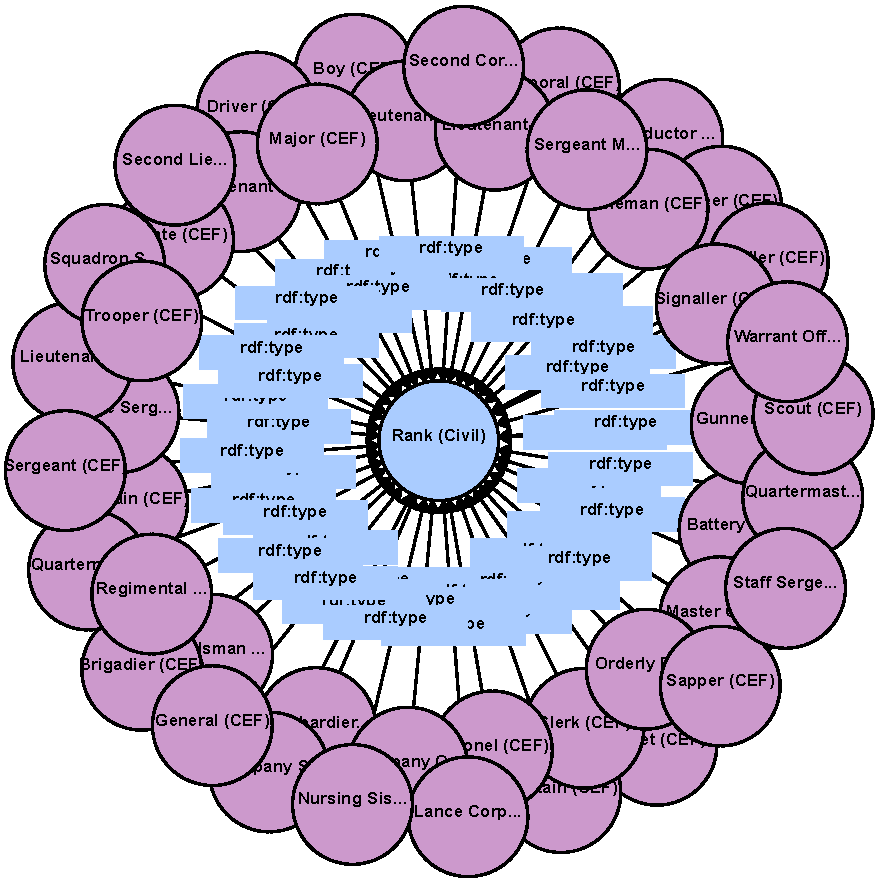
\includegraphics[width=8cm]{figures/code-list-visualized}
\caption{Visualization of a simple code list embedded in the Military Ontology v1.1 \cite{military_ontology}}
\label{fig:code-list-visualized}
%\vspace{-2mm}
\end{figure}

%There exist two common approaches to publishing a code list: 1) 
Aside such ontology-embedded structures, 
%sometimes also called \emph{value sets} \cite{alanrector}, 
the term `code list' is used for certain stand-alone datasets. %modeled using the SKOS vocabulary \cite{DBLP:journals/corr/abs-1801-04479}. 
Stand-alone code lists are being used, among others, in connection with government data %fiscal data where they have been defined as lists of values in a predefined set that can be used in metadata and that help metadata creators in selecting from a set of descriptors, thereby enhancing consistency and helping to avoid errors 
\cite{guide_code_list}, and modeled with the help of
%While some studies address the representation of code lists within specific domains using 
the SKOS vocabulary \cite{miles2009skos}. 
A typical applied case, e.g., in fiscal open budget data \cite{DBLP:conf/smap/FilippidisKKIB16}, is the association of code lists with dimension properties of a multi-dimensional dataset conforming to the Data Cube\footnote{\url{https://www.w3.org/TR/vocab-data-cube/}} vocabulary \cite{obeu_dcv}.

While the structural patterns and lexical conventions of embedded vs.~stand-alone code lists differ, it seems worthwhile not only to analyze embedded code lists but also to expose them as independent resources, augmented with features that are common for stand-alone code lists. 

%we are unaware of any prior research that would systematically retrieve, extract and document \emph{code lists embedded in ontologies} in order to facilitate their reuse even across the detailed domains.
%focus on the usage of code lists across domains while also taking into account both mentioned code list specification modes.

%Both can be characterized by the typical structural (and sometimes also lexical) patterns, which could be expressed as SPARQL queries to be used to query vocabulary catalog endpoints and individual knowledge graphs. 

The most tangible contribution of our research is a collection of \emph{SPARQL queries} performing the extraction of embedded code lists from ontologies, currently from the Linked Open Vocabularies knowledge base  (LOV) \cite{DBLP:journals/semweb/VandenbusscheAP17}, a web application (named Code List Analyzer) that allows browsing candidate code lists, a dataset of code lists and scripts to reproduce the results.
%Additional SPARQL queries can then be applied to a knowledge graph (we so far experimented with DBpedia) that would also contain code lists embedded in it.

%For the embedded code lists, we quantify their degree of adoption in comparison to the usage of their respective properties.

Given a broader perspective, we analyze embedded code lists from three different angles:
\begin{enumerate}
    \item As sets of RDF resources following some common \emph{graph patterns} in the ontology.%, common for all of its members.
    \item As sets of \emph{ontological universals}. We hypothesize (and the subsequent analysis described in this paper confirmed) that the codes of embedded code lists can pre-dominantly be characterized as ontological universals, i.e., generic concepts that can be instantiated (even if the instantiation cannot happen due to their incidental syntactic encoding by individuals), in contrast to particulars, which cannot have instances (under any circumstances). For this reason, we will discuss in more detail -- as a contextual framing rather than in direct connection to the empirical research presented as the core contribution of the paper -- how concepts can be represented using RDF/OWL.
    \item As sets of \emph{syntactic individuals}. We thus, beyond extracting code lists using the graph context, also carry out an exhaustive examination of all syntactic individuals present in LOV ontologies, and attempt to characterize their role, which can also be different than that of code list codes.
\end{enumerate}

The remaining parts of this paper are organized as follows. 
%In Section 2 we review three structural parts of the semantic web knowledge representation: ontology schemas, code lists, and knowledge graphs, at a general level.  
In Section \ref{s:codelist-def} we start from an authoritative definition of code list from EU public service guidelines as well as from past research on OWL patterns and attempt to derive from both a new formulation of versatile patterns characterizing embedded code lists in ontologies. 
In Section \ref{s:codelistanalyzer} we present an operational set of SPARQL queries based on those patterns, employed for browsing embedded code lists, the enabling tool (Code List Analyzer), and the results achieved when applying this inventory on the LOV ontology collection.
Section \ref{s:skos_codelist_collecting} explains how we extract code lists and `SKOSify' them for better coherence and interoperability.
In Section \ref{s:repr} we first demonstrate the dominant nature of embedded codes as ontological universals, and consequently discuss three alternatives for representing universals (or concepts) on the Semantic Web.
Section \ref{s:analysis_code_list_modeling_practice} describes a bottom-up analysis complementary to that from Section \ref{s:codelistanalyzer}; it starts from the set of all individuals inside all vocabularies, gradually partitioning their space by distinctive features, and, eventually, mapping these features to patterns from Section \ref{s:codelist-def}.
Section \ref{s:discussion} consists of a discussion of both quantitative and qualitative results from the previous analysis.
Section \ref{s:related} provides a comparison with related research.
Finally, Section \ref{s:conclusion} wraps up the paper.
%and outlines the directions for future work.